\documentclass[a4paper]{article} 

%中文环境设置
\usepackage{xeCJK} 
\usepackage{indentfirst}
\setlength{\parindent}{2em}
\usepackage{enumitem}

\usepackage{abstract}
\renewcommand{\abstractname}{摘要}
\providecommand{\keywords}[1]{\textbf{\textit{关键词}} #1}

\setCJKmainfont{STSong} % 中文主字体设置 

\usepackage[colorlinks,linkcolor=blue, citecolor=blue]{hyperref}

% 常用宏包
\usepackage{float}
\usepackage{stfloats}
\usepackage{graphicx}
\usepackage{color}
\usepackage{supertabular}

% 代码环境设置
\usepackage{listings}
\lstset{
	columns=fullflexible,
 	frame=single,
 	breaklines=true,
}
\definecolor{lightgray}{gray}{0.9}
\newcommand{\inlinecode}[2]{\colorbox{lightgray}{\lstinline[language=#1]$#2$}}

% 页面段落设置
\usepackage{multicol}
\usepackage{geometry}
\geometry{left=3.18cm, right=3.18cm, top=2.54cm, bottom=2.54cm}
\linespread{1.3}
%\setlength{\parskip}{0.5em} 

% 数学环境设置
\usepackage{amsmath}
\usepackage{amssymb}
\usepackage{amsthm}
\usepackage{amsfonts}
\newtheorem{myDef}{Definition} 
\newtheorem{myThm}{Theorem}
\newtheorem{myProp}{Property}

\begin{document} 
\title{插值法实验题}
\author{吴佳龙 2018013418}
\date{}
\maketitle

\begin{abstract}
	结合理论分析和编程计算,运用不同算法对一特定函数进行插值,并观察了 Runge 现象。运用的插值方法分别为 Lagrange 插值、分段线性插值、三次自然样条插值。
\end{abstract}

%\keywords{one, two, three, four}

\begin{multicols}{2}

\begin{section}{问题}

	设 $$f(x)=\frac{1}{1+25 x^{2}}, x \in[-1,1]$$ 取 $x_{j}=-1+\frac{2 j}{n}, j=0,1, \cdots, n$。
	
	取适当的 $n$,试求出 $n$ 次 Lagrange 插值多项式 $L_n(x)$、分段线性插值函数 $I_1^h(x)$ 和三次样条插值函数 $S_3^h(x)$ (采用自然边界条件),画出他们的图像,并对结果做一个比较说明。

\end{section}

\begin{section}{Lagrange 插值}
	
	\begin{subsection}{算法原理}
		
		取基函数 $$l_{k}(x)=\prod_{i=0, i \neq k}^{n} \frac{x-x_{i}}{x_{k}-x_{i}}, \quad k=0,1, \cdots, n$$
		
		令 $$p_{n}(x)=\sum_{k=0}^{n} y_{k} l_{k}(x)$$ 其中 $y_{k}=f\left(x_{k}\right)$。
		
		容易验证 $p_{n}\left(x_{i}\right)=y_{i}=f\left(x_{i}\right)$ 且 $n$ 次插值多项式具有唯一性。
		
		\begin{subsubsection}{误差估计}
			
			\begin{myThm}
				
				记步长 $ h=\max _{1 \leq j \leq n}\left|x_{j}-x_{j-1}\right| $,则插值余项满足 $$\left\|R_{n}(f)\right\|_{\infty} \equiv\left\|f-L_{n}(f)\right\|_{\infty} \leq \frac{h^{n+1} \left\|f^{(n+1)}\right\|_{\infty}}{4(n+1)}$$
				
			\end{myThm}
			
		\end{subsubsection}
		
		\begin{subsubsection}{收敛性}
		
			由以上定理可知:若被插值函数的任意阶导数一致有界,那么插值多项式可以收敛到被插值函数。
			
			一般情况下,这种条件难以达到。例如本次实验中的被插值函数就是 Runge 于 1901 年所研究的例子,插值多项式在区间端点附近的振荡现象被称为 Runge 现象。
			
		\end{subsubsection}
		
	\end{subsection}

	\begin{subsection}{算法实现}
	
		Lagrange 插值的 MATLAB 实现如下:
		
		\begin{lstlisting}[language=Matlab]
function coeff = myLagrangeInterp(x,y)
% lagrange 插值法
% 返回格式:coeff 为 (1,n+1) 大小的向量,分别表示从常数项到最高次项的系数
[~,n] = size(x);
n = n-1;
coeff = zeros(1,n+1);
l = zeros(n+1,n+1); % 基函数
for i = 1:n+1
    l(i,1) = 1; prod = 1;
    for j = 1:n+1
        if (i==j)
            continue
        end
        l(i,:) = [0, l(i, 1:end-1)] - x(j)*l(i,:);  
        prod = prod*(x(i)-x(j));
    end
    coeff = coeff + y(i)*l(i,:)/prod;
end
end
		\end{lstlisting}

	\end{subsection}

\end{section}

\begin{section}{分段线性插值}
	
	\begin{subsection}{算法原理}
		
		令 $$I_h(x) = y_j {x_{j+1}-x\over h_j} + y_{j+1} {x-x_j\over h_j}, x\in [x_j, x_{j+1}]$$ 则 $I_h(x)$ 为 $f(x)$ 的分段线性插值函数,满足:
		
		\begin{itemize}
  			\item $I_h \in C[a,b]$
  			\item $I_h(x_j) = f(x_j)$
  			\item 在 $[x_j, x_{j+1}]$ 上是线性多项式
		\end{itemize}
		
		\begin{subsubsection}{误差估计}
			
			\begin{myThm}
				
				设 $f\in C^2[a,b]$,那么有 $$\left\|f-I_h\right\|_{\infty} \leq {h^2\over 8} \left\|f^{\prime \prime}\right\|_{\infty}$$
				
			\end{myThm}
			
		\end{subsubsection}
		
		\begin{subsubsection}{收敛性}
			
			利用连续模的性质,可得收敛性定理:
			
			\begin{myThm}
				
				设 $f\in C[a,b]$,那么当 $h \rightarrow 0$ 时,$I_{h} \rightrightarrows f$ .
				
			\end{myThm}

				
		\end{subsubsection}

		
	\end{subsection}

	\begin{subsection}{算法实现}
		
		分段线性插值的 MATLAB 实现如下:
		
		\begin{lstlisting}[language=Matlab]
function coeff = myLinearInterp(x,y)
% 分段线性插值
% 返回值 coeff 为 (n,2) 的矩阵,分别表示 n 段的常数项和一次项系数
[~,n] = size(x);
n = n-1;
coeff = zeros(n,2);
for i = 1:n
    h = x(i+1)-x(i);
    coeff(i,1) = (y(i)*x(i+1)-y(i+1)*x(i))/h;
    coeff(i,2) = (y(i+1)-y(i))/h;
end
		\end{lstlisting}
		
	\end{subsection}
	
\end{section}

\begin{section}{三次样条插值}
	
	\begin{subsection}{算法原理}
		
		若函数 $S_(x)$ 满足:
		
		\begin{itemize}
			\item $S\in C^2[a,b]$
			\item $S$ 在 $[x_j,x_{j+1}]$ 上是三次多项式 
		\end{itemize} 
		则称 $S$ 是一个\textbf{三次样条函数}。
		
		若 $S$ 满足 $S(x_j) = f(x_j)$ ,则称 $S$ 为 $f$ 的 \textbf{三次样条插值函数}。更进一步地,$S$ 满足\textbf{自然边界条件} $$S^{\prime\prime}(x_0) = S^{\prime\prime}(x_n) = 0$$ 则称为\textbf{自然样条函数}。

		三次样条插值函数可以通过转角方程、三弯矩方程、B-样条函数等方法求解。
		
		\begin{subsubsection}{转角方程}
		
			假定 $S^{\prime \prime}(x_j) = M_j$ 已知,则通过插值条件 $S(x_j) = f(x_j)$ 可以得到:
			
			$$\begin{aligned} S(x)=& M_{j} \frac{\left(x_{j+1}-x\right)^{3}}{6 h_{j}}+M_{j+1} \frac{\left(x-x_{j}\right)^{3}}{6 h_{j}}\\&+\left(f\left(x_{j}\right)-\frac{M_{j} h_{j}^{2}}{6}\right) \frac{x_{j+1}-x}{h_{j}} \\ &+\left(f\left(x_{j+1}\right)-\frac{M_{j+1} h_{j}^{2}}{6}\right) \frac{x-x_{j}}{h_{j}}, \quad x \in\left[x_{j}, x_{j+1}\right] \end{aligned}$$
			
			为确定 $M_j$,可利用 $S^{\prime}$ 的连续性,得到线性方程组:$$\mu_{i} M_{j-1}+2 M_{j}+\lambda_{j} M_{j+1}=d_{j}, \quad j=1,2 \cdots, n-1$$ 其中 $$\begin{aligned} \mu_{j}&=\frac{h_{j-1}}{h_{j-1}+h_{j}}, \\ \quad \lambda_{j}&=1-\mu_{j}=\frac{h_{j}}{h_{j-1}+h_{j}} \\ \quad d_{j}&=6 f\left[x_{j-1}, x_{j}, x_{j+1}\right] \end{aligned}$$
			
			增加自然边界条件 $M_0 = M_n = 0$,方程组变为:
			
			\begin{tiny}
			$$\left[\begin{array}{ccccc}{2} & {\lambda_{1}} & {} & {} & {} \\ {\mu_{2}} & {2} & {\lambda_{2}} & {} & {} \\ {} & {\ddots} & {\ddots} & {\ddots} & {} \\ {} & {} & {\mu_{n-2}} & {2} & {\lambda_{n-2}} \\ {} & {} & {} & {\mu_{n-1}} & {2}\end{array}\right]\left[\begin{array}{c}{M_{1}} \\ {M_{2}} \\ {\vdots} \\ {M_{n-2}} \\ {M_{n-1}}\end{array}\right]=\left[\begin{array}{c}{d_{1}} \\ {d_{2}} \\ {\vdots} \\ {d_{n-2}} \\ {d_{n-1}}\end{array}\right]$$
			\end{tiny}
			
		\end{subsubsection}
		
	\end{subsection}

	\begin{subsection}{算法实现}
		
		三次自然样条插值的 MATLAB 实现如下:
		
		\begin{lstlisting}[language=Matlab]
function coeff = mySplineInterp(x,y)
% 三次自然样条插值
% 返回值 coeff 为 (n,4) 的矩阵,分别表示 n 段的常数项到三次项系数
[~,n] = size(x);
n = n-1;
coeff = zeros(n,4);
h = x(2:end) - x(1:end-1);
mu = h(1:end-1)./(h(1:end-1)+h(2:end));
lambda = 1-mu;
df = (y(2:end)-y(1:end-1))./(x(2:end)-x(1:end-1));
d = 6*(df(2:end)-df(1:end-1))./(x(3:end)-x(1:end-2));
% 转角方程
A = 2*eye(n-1)+diag(mu(2:end), 1)+diag(lambda(1:end-1), -1);
b = d;
M = [ 0; A\(b'); 0];
for j = 1:n
    coeff(j,:) = coeff(j,:) + [x(j+1)^3, -3*x(j+1)^2, 3*x(j+1), -1]*M(j)/6/h(j);
    coeff(j,:) = coeff(j,:) + [-x(j)^3, 3*x(j)^2, -3*x(j), 1]*M(j+1)/6/h(j);
    coeff(j,:) = coeff(j,:) + [x(j+1), -1, 0, 0]*(y(j)-M(j)*h(j)^2 / 6) / h(j);
    coeff(j,:) = coeff(j,:) + [-x(j), 1, 0, 0]*(y(j+1)-M(j+1)*h(j)^2 / 6) / h(j);
end
end
		\end{lstlisting}
		
	\end{subsection}
	
\end{section}

\begin{section}{方法比较}
	
	\begin{subsection}{误差}
	
		选取不同的 $n$,计算不同插值函数的误差 $\left\|f-\right\|_{\infty}$  如下:
		
		\begin{table}[H]
		\begin{tabular}{c|c|c|l}
		\hline
		                              &  $L_{n}(f)$              & $I_h(f)$                        & $S(f)$   \\ \hline
		$n=5$                         & 0.432692                  & 0.500000                      & 0.423482 \\
		$n=10$                        & 0.326236                  & 0.067431                      & 0.010959 \\
		$n=15$                        & 0.249218                  & 0.100000                      & 0.030891 \\
		$n=20$                        & 58.278126                 & 0.041538                      & 0.002310 \\
		\multicolumn{1}{l|}{$n=100$}  & \multicolumn{1}{l|}{1e42} & \multicolumn{1}{l|}{0.002457} & 0.000025 \\
		\multicolumn{1}{l|}{$n=1000$} & \multicolumn{1}{l|}{NaN}  & \multicolumn{1}{l|}{0.000006} & 0.000000 \\ \hline
		\end{tabular}
		\end{table}	
		
	\end{subsection}
	
	\begin{subsection}{图像}
	
		选取 $n=10$,绘制原函数和插值函数的图像如图 \ref{compare} 所示。
		
		\begin{figure*}[ht]
			\centering
			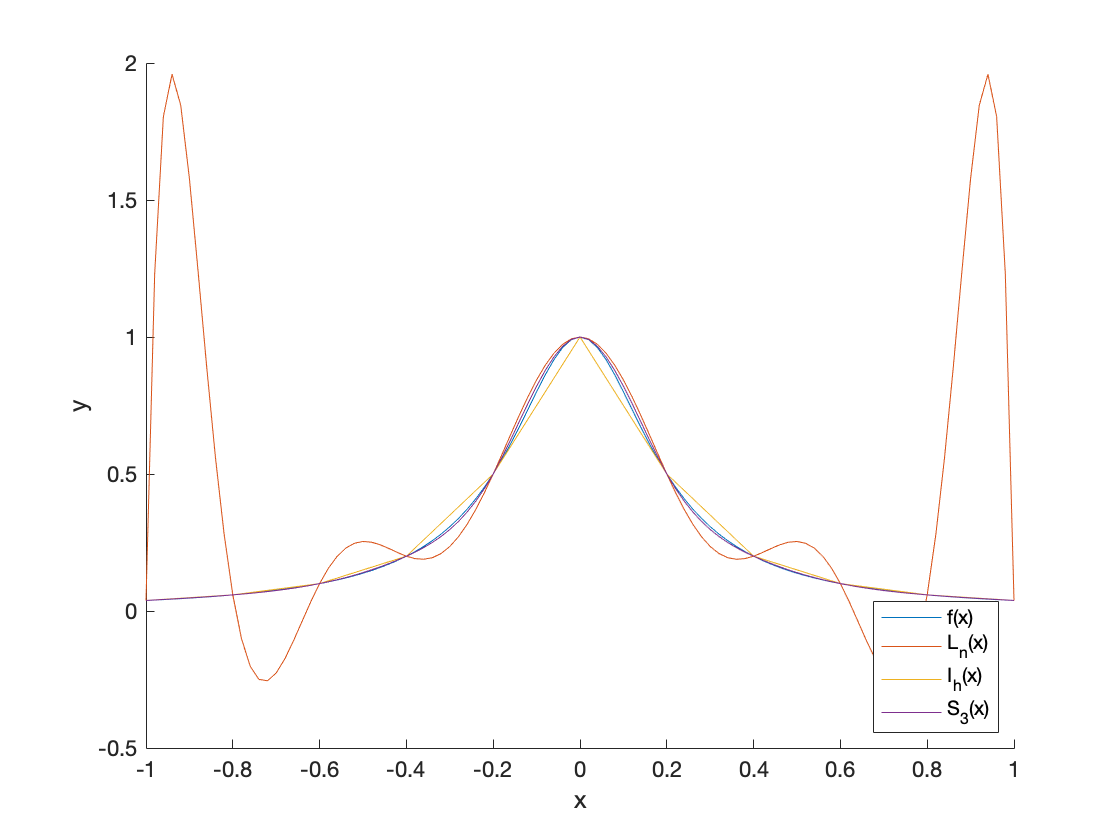
\includegraphics[width = 0.9\textwidth]{img/compare.png} 
			\caption{原函数和插值函数的图像 $n=10$}
			\label{compare} 
		\end{figure*}	
		
		\begin{subsubsection}{Runge 现象}
		
			分别选取 $n=6, 10, 14$,绘制 $L_n(x)$ 的图像,观察 Runge 现象如图 \ref{runge} 所示。
			
			\begin{figure*}[ht]
				\centering
				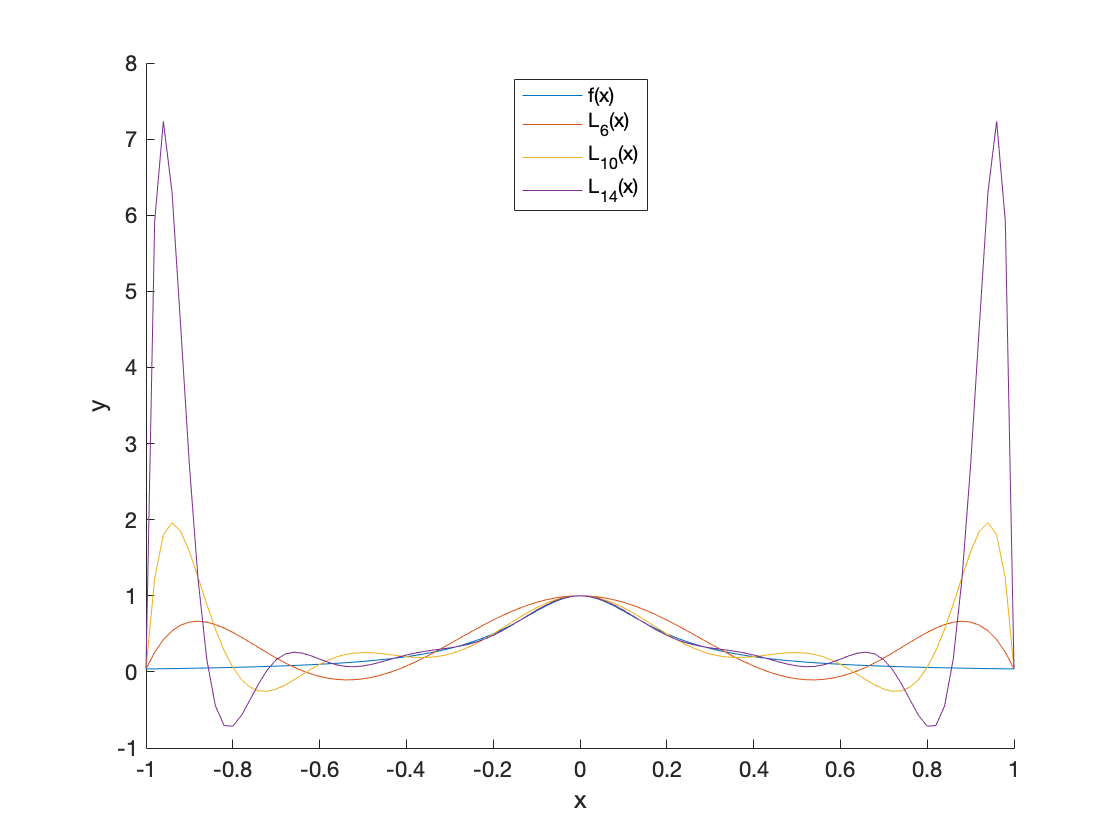
\includegraphics[width = 0.9\textwidth]{img/runge.png} 
				\caption{Runge 现象 $n=6,10,14$}
				\label{runge} 
			\end{figure*}	 
			
		\end{subsubsection}
		
	\end{subsection}
	
	\begin{subsection}{结论}
	
		随着 $n$ 的增加,Lagrange 插值多项式对于本次实验中的被插值函数不收敛,且出现了 Runge 现象。
		
		分段线性插值函数和三次自然样条插值函数都收敛到被插值函数,但是分段线性插值函数的导数在采样点是不连续的,且三次样条插值函数的误差和收敛速度都由于分段线性插值函数。
		
	\end{subsection}
	
\end{section}
	
\begin{section}{总结}
	
	本次实验对于几种不同的插值方法的算法进行了理论分析和编程计算,作出图像并比较了它们的结果。
	
	结果符合预期:观察到 Lagrange 插值法的Runge现象;分段线性插值函数和三次样条插值函数都收敛到被插值函数,且三次样条插值函数的表现优于分段线性插值函数。
	
\end{section}

\end{multicols}



%\bibliographystyle{unsrt}
%\bibliography{ref.bib}

%\begin{thebibliography}{99}    %参考文献开始
%	\bibitem{ml}周志华. 机器学习[M]. 清华大学出版社, 2016.   
%\end{thebibliography}	

\end{document}

